%to do
\section{Background and Motivation}
\label{sec:background}
If we execute data intensive workloads in clouds, the performance is
expected to be unacceptable because I/O performance of shared storage in clouds
are fairly slow (in Section \ref{ssec:IO_performance_in_clouds}). 
However, our analysis of data intensive workloads on HPC systems, we found
that a number of applications have temporal I/O locality (in Section
\ref{ssec:data_access_locality}). These I/O workloads can be accelerated even on
clouds where shared storage performance is low (in Section
\ref{ssec:network_s3}) if we use our cloud-based burst buffer system works as an
\emph{on-demand remote cache space}. 


\begin{comment}
\subsection{Cloud Computing}
\begin{figure}
\centering
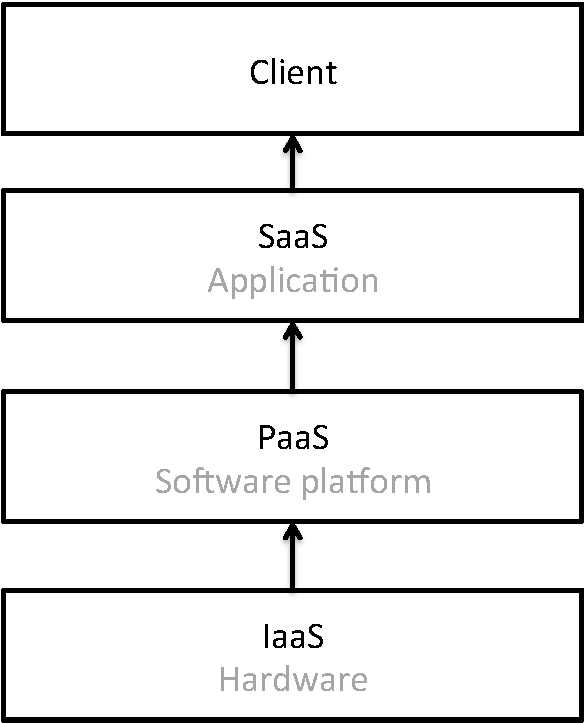
\includegraphics[width=4cm]{img/cloud_models.pdf}
\caption{the relationship of different cloud models}
\label{background:cloud models}
\end{figure}

Cloud computing refers to a model that cloud vendors provide user IT resources and charge them for
the resources they used.
Cloud vendors can offer hardware resources including CPU, memory, hard disk, network and software
resources OS, software suits and applications.
Cloud computing majorly can be classified into following three kinds of models:
\begin{enumerate}
  \item Infrastructure as a service (IaaS): cloud vendors provide only raw machines(physical or
  virtual machine), user need to set up the whole software environment including OS.
  \item Platform as a service (PaaS): in this model, cloud vendors provide
  hardware as well as software platform. Users can use it as a common computer and run applications on the platform.
  Amazon EC2 provides PaaS.
  \item Software as a service (SaaS): Cloud vendors provide a certain applications. Users don't need
  to configure the software themselves.
\end{enumerate}
The relationship of different cloud models can be shown as Figure~.\ref{background:cloud models}

Cloud computing can have following benefits:
\begin{itemize}
  \item Users don't need to care about the machine placement and maintenance.
  \item Users don't need a large number of machines to meet a temporally request peek and idle for
  the other time, Since cloud instances can set up in a few minutes when the request peek occurs.
  \item Users don't need to pay for expensive hardware and software, they just need to pay for what
  they used.
\end{itemize}
\end{comment}
\subsection{I/O Performance in Cloud Storage}
\label{ssec:IO_performance_in_clouds}

% \kento{There is no topic sentence in this subsection. Why did you write this
% Subection ? why do you compare  Interconnection Network vs. Shared Storage}
% In public cloud system, although shared storage cannot achieve a high performance, the
% interconnection network between compute nodes usually has a high bandwidth.
% Our proposal system takes advantage of high throughput of interconnection network between compute
% nodes inside cloud system to burst I/O throughput.
% In order to show the difference of throughput between Amazon S3 and interconnection network between
% compute nodes.
% First we measured the sequential I/O performance of Amazon S3, we measured read and write throughput
% with different size of compute nodes, and we also measured the two I/O pattern performance which
% will compute nodes shared the same file and each compute nodes access to different file.
% Figure~\ref{background:amazon s3 throughput} shows the result, we can see that compare to modern parallel file systems in HPC systems, for example TSUBAME lustre can achieve 6-8GB/s\cite{checkpointing}
%  Amazon S3 cannot achieve a high throughput, and the value is
% quite unstable.
% Many previous studies also measured the I/O throughput in clouds
% \cite{Chiba,Transactions_a_la_carte, Interactive_Use_of_Cloud_Services,Amazon_S3_for_Science_Grids,
% anevaluation} and got a similar result.
% \kento{Because you already evaluated S3 performance, I do not think this
% paragraph is necessary. Instead, please use these sentences to support your
% results, and show the results are consistent to evaluations done by others}
%  
% However, when we look at the point to point communication throughput between two compute nodes
% inside Amazon EC2,
% We measure this interconnection network by using Iperf [14].
% \kento{What does the ``inside'' mean ? please describe what did you measure}
% Figure.~\ref{background:amazon throughput} shows a comparison of Amazon Interconnection Network
% throughput and Amazon S3 throughput, although we only show the result up to 8 pairs of nodes
% \kento{Because you did not describe how to measure the performance,
% ``pairs'' is not unknown}, each node achieved only 135MB/s (1GBit/s), the
% influence between nodes is extremely small, figure shows a perfect linear line also a strong scalability.
% \kento{It's too detailed. And Should be mentioned before showing results}.
% When we running the
% benchmark, many other users were also running applications on Amazon, so we can assume that highest
% throughput 1GB/s (8Gbit/s) shown in Figure.~\ref{background:amazon throughput} is not the
% maximum bandwidth of interconnection network in Amazon EC2 \kento{Why do you
% mention this ? If you want to say ``this results is not trustful because other
% applications were running'', please remove this figure and this subsection.
% Instead, you should mention ``Even with other applications are running, the
% performance is still better than S3'' . But, in fat tree topology, almost peak
% throughput can be achieved even if other applications are running like in
% TSUBAME. So I do not think your expectation is true}.
% As Figure.~\ref{background:amazon throughput} shows, Interconnection Network throughput inside
% Amazon EC2 is proportional to numbers of nodes used, on the contrary, Amazon S3 throughput is much
% lower than it, and unstable.
% Also we can find that all nodes access to the same file is slower than access to different file,
% it is because Amazon S3 will distribute different file over machines to increase I/O throughput,
% access to the same file will be limited by S3 server machine bandwidth, and will cause connection
% conflict.
% \kento{Please mention ``so what?''. Why did you compare network(interconnection
% network) and storage(S3) ? People will think this comparison is unfair, and no
% meaning unless you mention that. This subsection looks weird to me because this
% section does not have any ``topic sentence'' and ``so what ?'' sentence}
% 
% \begin{figure}[h]
% \centering 
% \subfigure[Amazon S3 read/write (N-1)]{
% \label{background:amazon s3 read write same file}
% 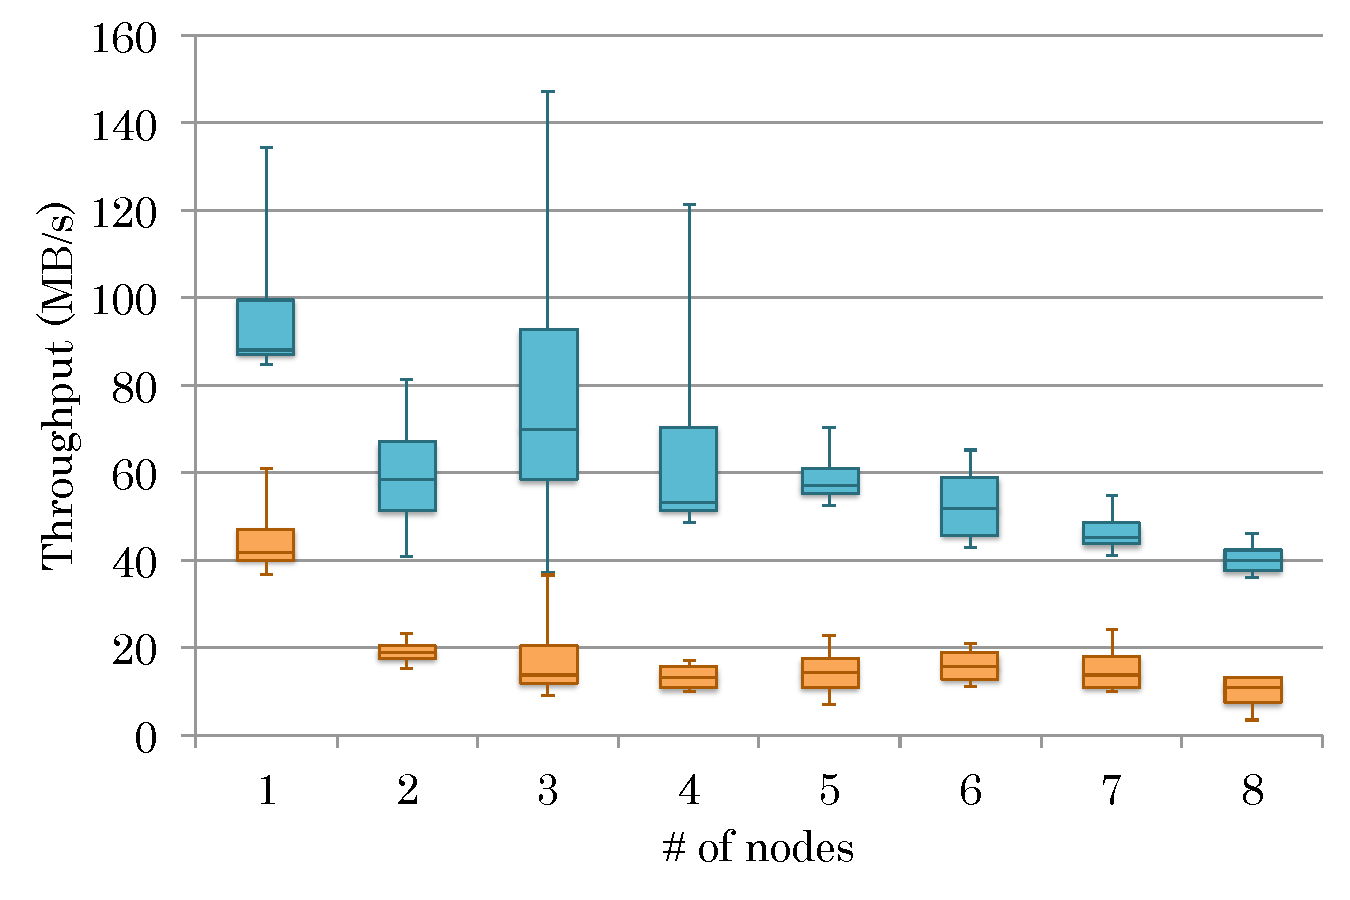
\includegraphics[width=4.1cm]{img/s3_read_write_same_file}}
% % \subfigure[Amazon S3 write (same file)]{
% % \label{background:amazon s3 write same file}
% % 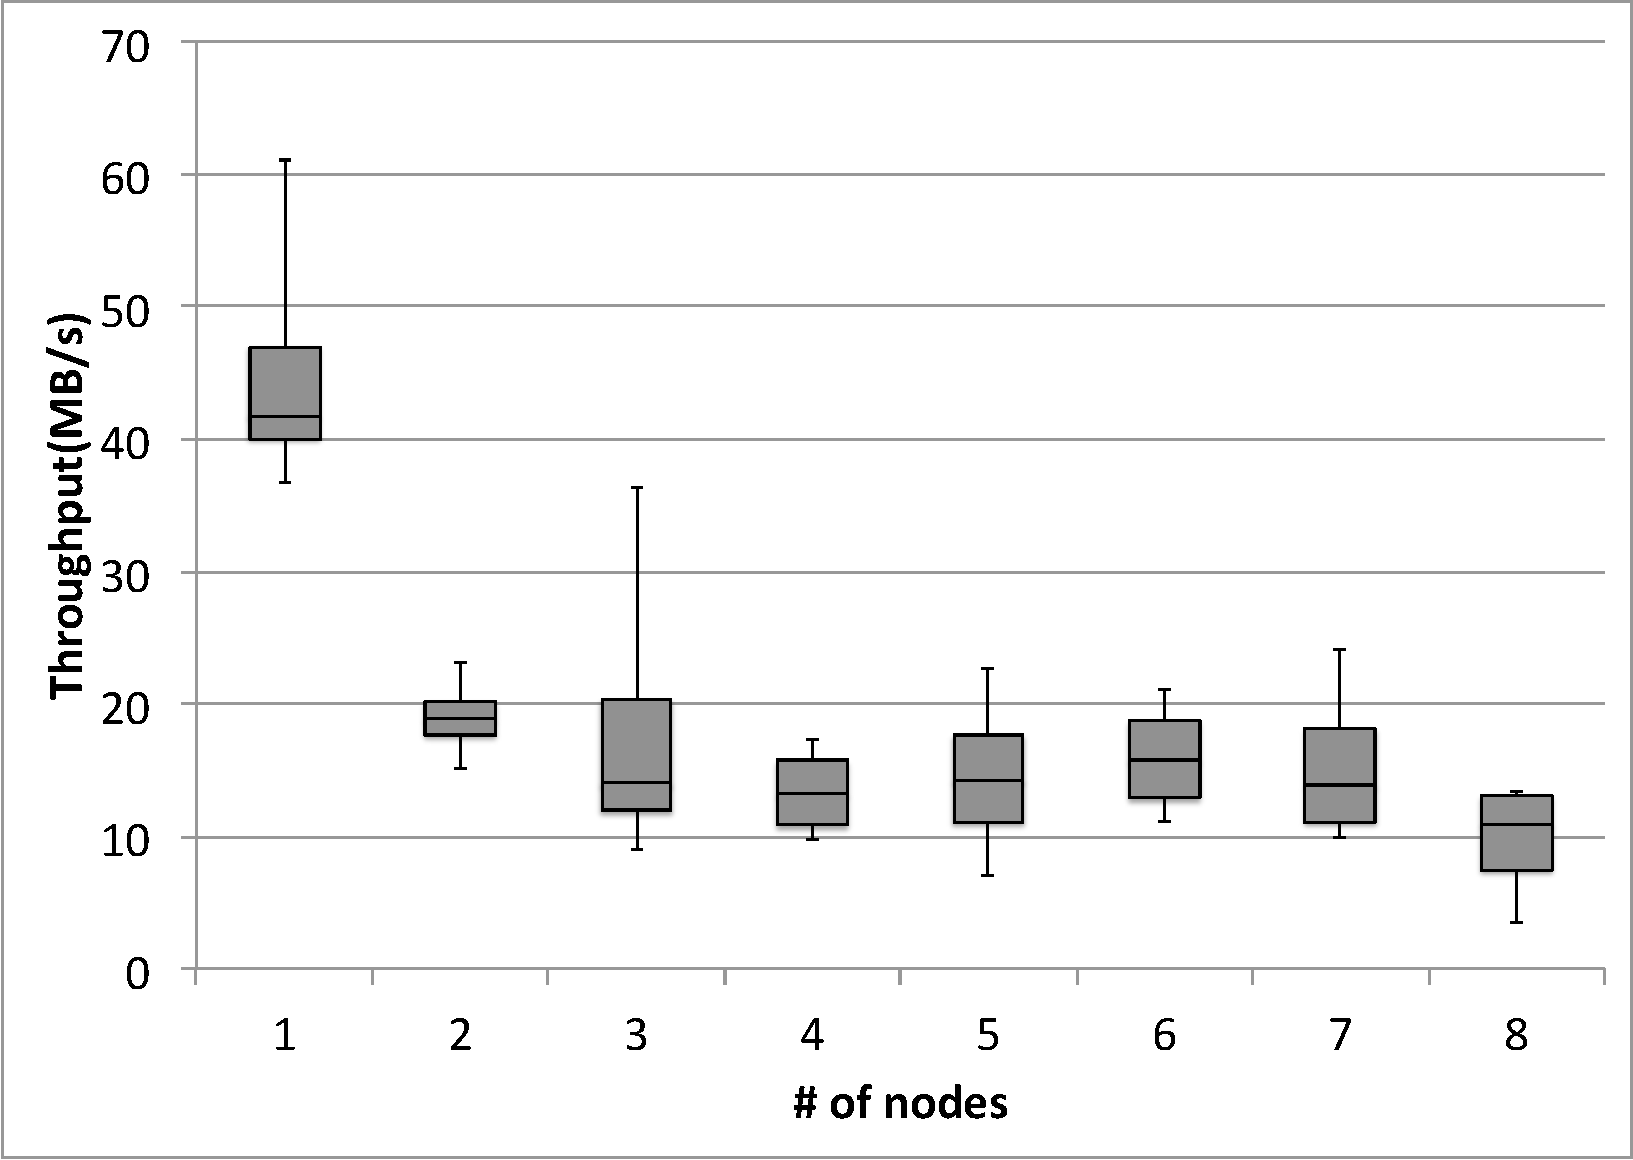
\includegraphics[width=4cm]{img/s3_write_same_file}}
% % \subfigure[Amazon S3 read (different file)]{
% % \label{background:amazon s3 read different file}
% % 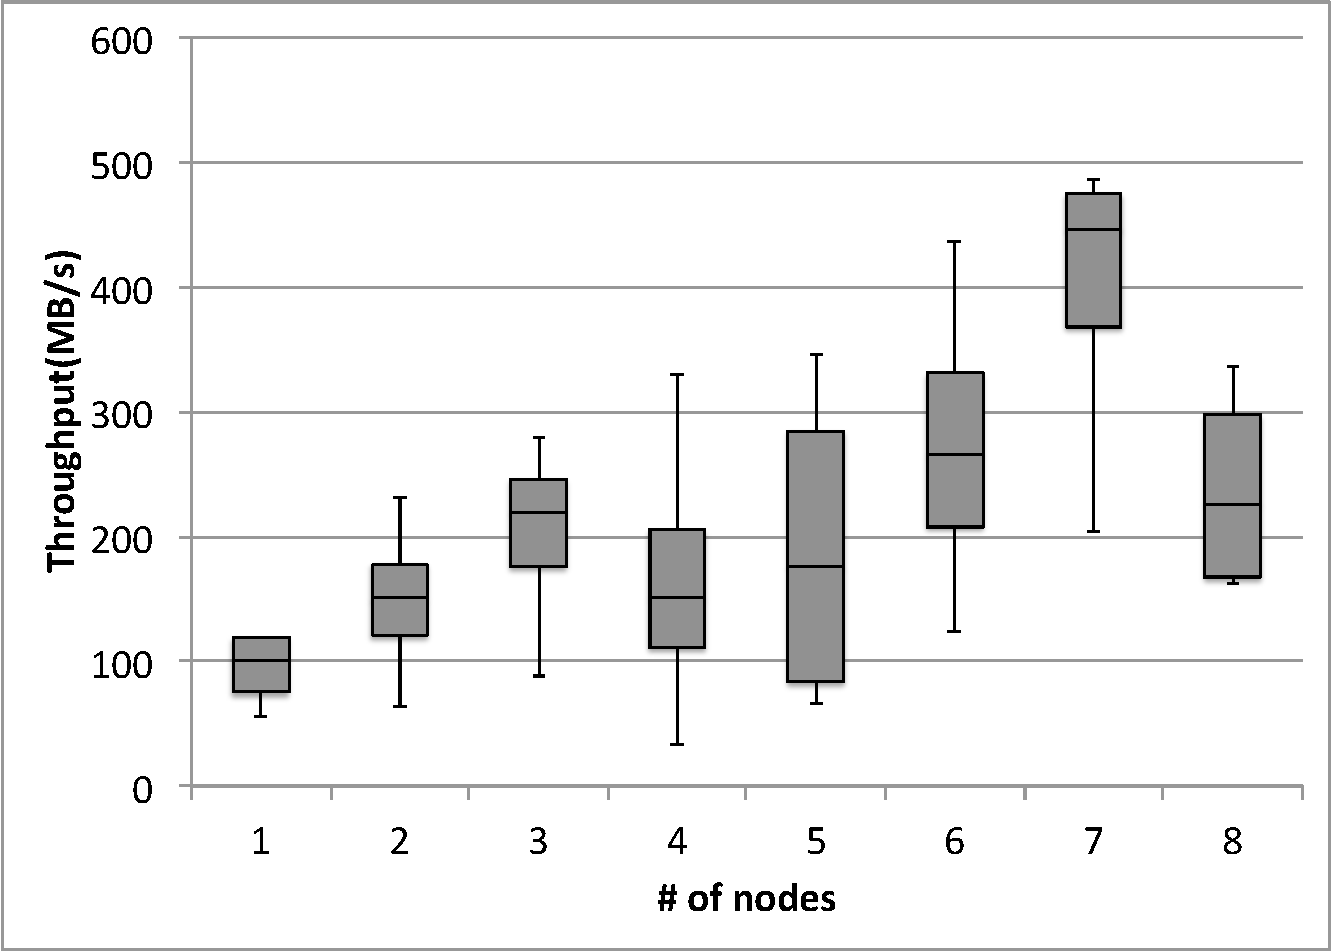
\includegraphics[width=4cm]{img/s3_read_different_file}}
% \subfigure[Amazon S3 read/write (N-N)]{
% \label{background:amazon s3 read write different file}
% 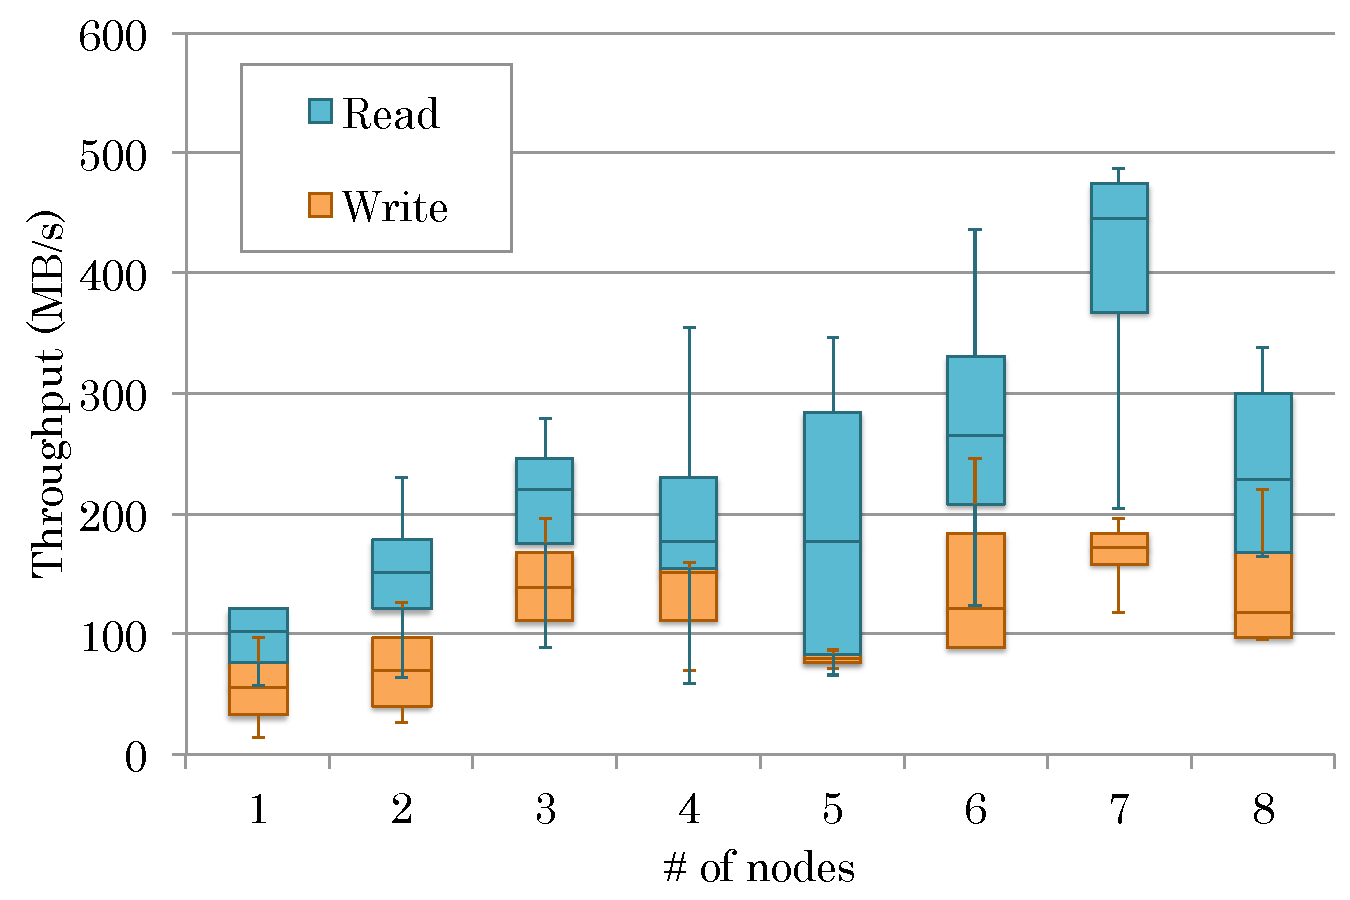
\includegraphics[width=4.1cm]{img/s3_read_write_different_file-2}}
% \caption{Amazon S3 I/O throughput}
% \label{background:amazon s3 throughput}
% \end{figure}
% 

\begin{figure}[t]
\centering
\label{background:amazon s3 read write same file}
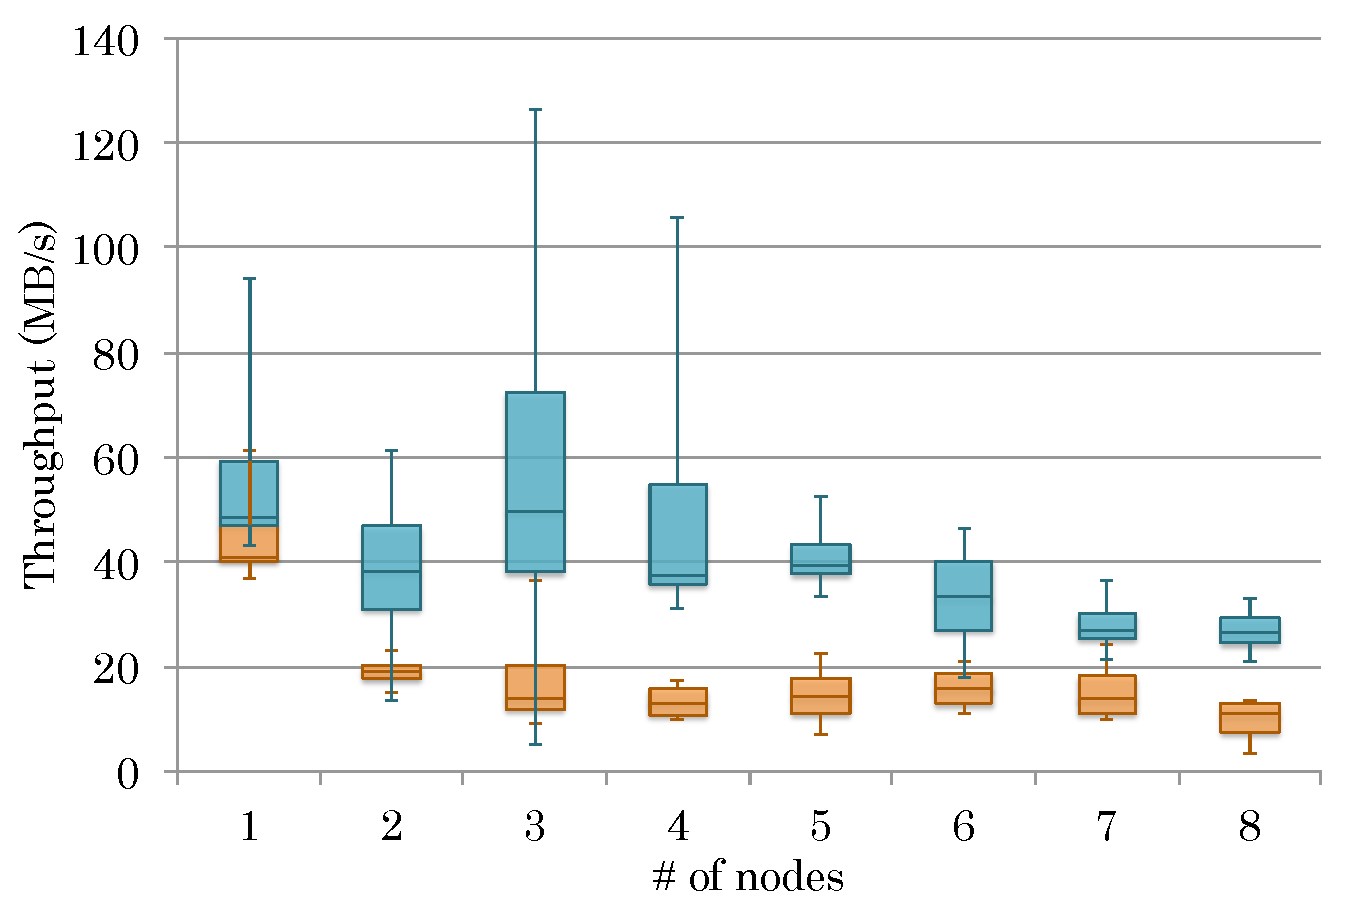
\includegraphics[width=8cm]{img/s3_read_same_file-2}
\caption{Amazon S3 read/write (N-1)}
\end{figure}

\begin{figure}[t]
\label{background:amazon s3 read write different file}
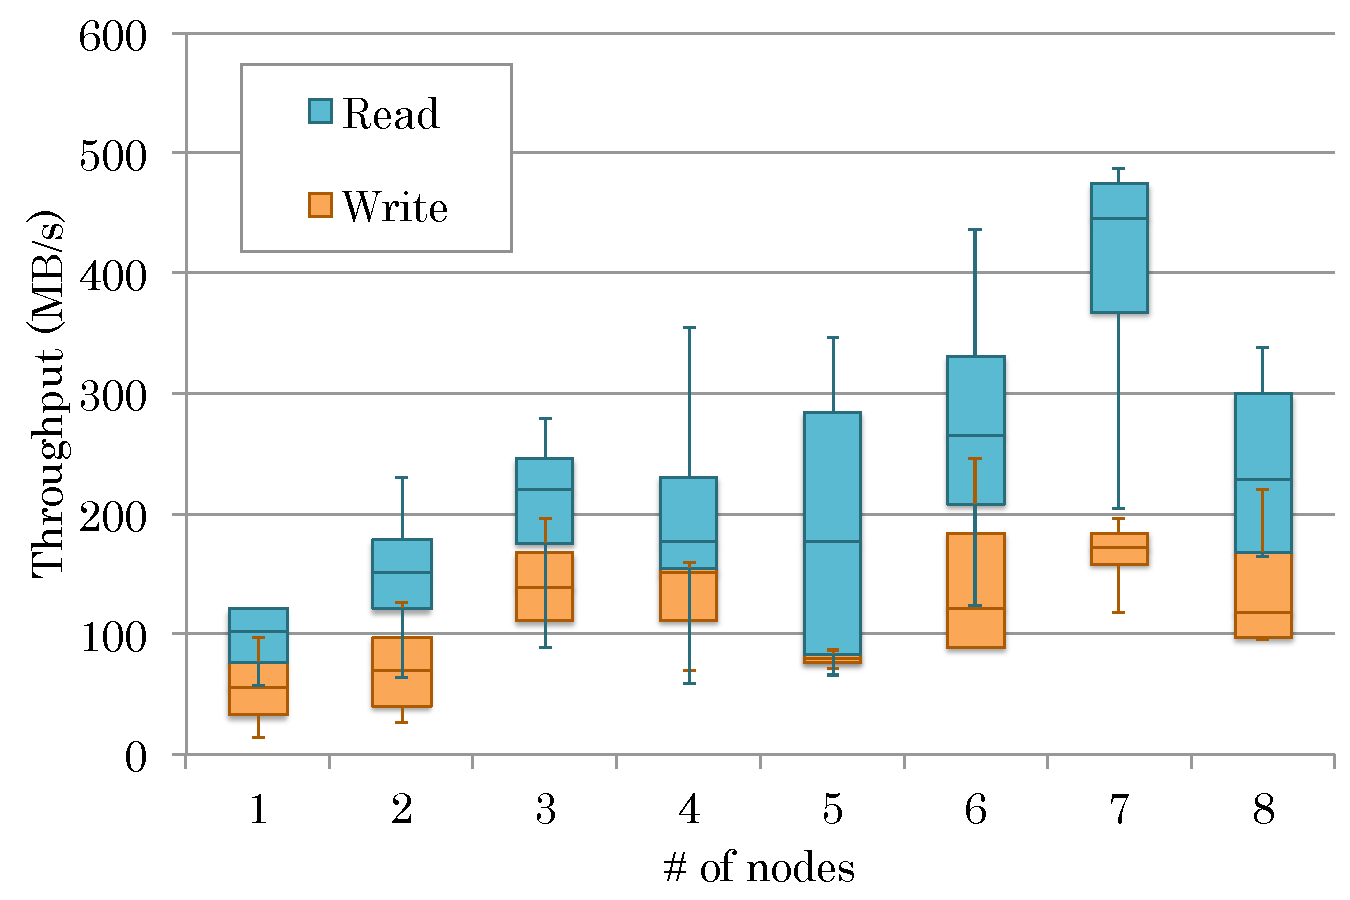
\includegraphics[width=8cm]{img/s3_read_write_different_file-2}
\caption{Amazon S3 I/O throughput (N-N)}
\end{figure}





The computational power in clouds enables the users to run high performance
scientific applications faster than ever, which have been making cloud
computing attractive to large scale scientific applications.
However if we run data intensive workloads, which read and write a huge amount
of data, the prolonged execution time can be unacceptable because of the low I/O
throughput in cloud storage.
\par
Figure \ref{background:amazon s3 read write same file} shows I/O throughputs
with different numbers of nodes which read or write to a single file, i.e.,
$N-1$ I/O.
As shown, the I/O throughputs are only 150 MB/s even in the best case of read,
which degrades performance of data intensive workloads. 
Figure \ref{background:amazon s3 read write different file} shows I/O
throughputs with different numbers of nodes which read or write to their
individual files, i.e., $N-N$ I/O. If each node read or write to their
individual files, we see improvement in scalability compared to $N-1$ I/O. 
However, the improvement is limited. Especially, write performance does not
scale to the number of nodes. From the figures, we also see that the I/O
performance is fairly unstable. Because typical data intensive applications consist of
processes which have dependency each other, prolonged I/O
operation due to the instability can propagate, and degrades the overall
performance \cite{montage, povray}.
There problems are also reported in existing studies \cite{Chiba,Transactions_a_la_carte, Interactive_Use_of_Cloud_Services,Amazon_S3_for_Science_Grids,
anevaluation}. 
Thus, new technology is required to achieve higher and more stable I/O
performance.

 



\subsection{Temporal I/O Locality in Data Intensive Workloads}
\label{ssec:data_access_locality}
\begin{comment}
add other kinds of application data locality details.
as more as possible
\end{comment}

\begin{table}
\centering
\begin{tabular}{|c|p{150pt}|}
\hline
\cellcolor{lightgray} Montage	&
 A portable software toolkit for constructing custom, science-grade mosaics by
 composing multiple astronomical images~\cite{montage}.\\\hline 
\cellcolor{lightgray} POV-Ray   &
 A ray tracing program which generates images
 from a text-based scene description~\cite{povray}.\\\hline
\cellcolor{lightgray} Supernovae &	
 A astronomical program that builds a catalogue of
objects from astronomical images using Source-Extractor\cite{SExtractor}, 
and find supernovae from the images in a CFITSIO data format \cite{fitsio}.
% a library of C and Fortran subroutines for reading and writing data files
%in FITS (Flexible Image Transport System) data format to find supernovae in a
% set of astronomical image.
\\ \hline
\end{tabular}
\caption{Real data intensive workflow applications}
\label{background:work flow applications}
\end{table}

\begin{figure}
\centering
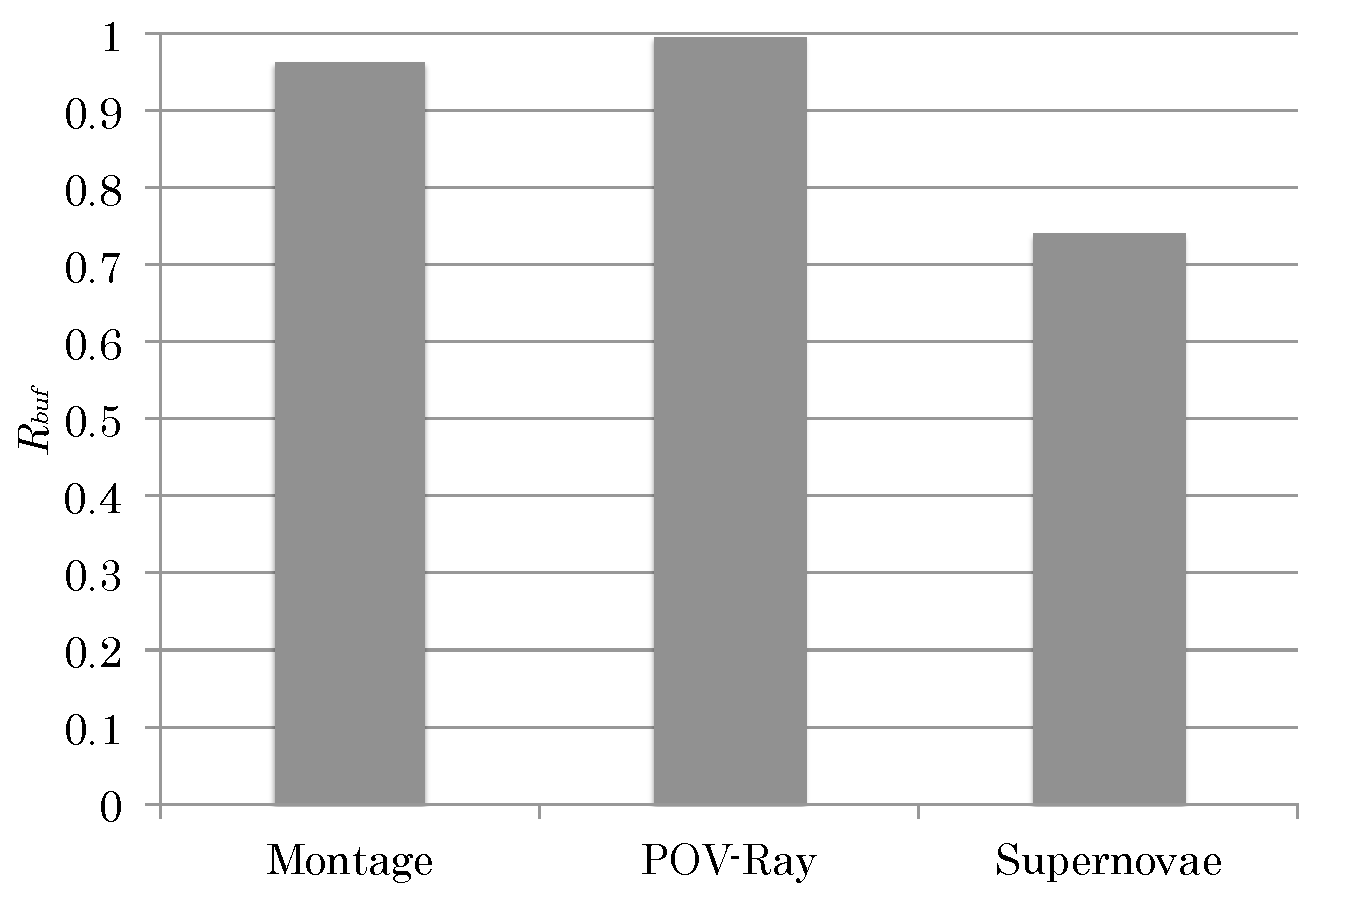
\includegraphics[width=8cm]{img/data_locality-2.pdf}
\caption{Temporal I/O locality in data intensive applications}
\label{background:data locality}
\end{figure}

%\kento{There is no topic sentence in this subse$ction. Why did you write this
%subection ? why do you describe data access locality}
% Since our proposal
% system buffer I/O data and as previous section shows the buffered data can be accessed in a high
% throughput, applications' data access locality will affect the performance gains by using our
% propose system greatly.
% Data locality is a phenomenon describing the same value, or related storage locations, being
% frequently accessed.
% Technology like cache, instruction prefetch for memory, or the advanced
% branch predictor at the pipelining of processors is based on this phenomenon.
% Many previous research investigated data locality of various
% applications including 
% mapreduce,\cite{Investigation_of_Data_Locality_in_MapReduce}, scientific
% \cite{Intrinsic_data_locality_of_modern_scientific_workloads},
% OLTP\cite{Data_locality_characterization_of_OLTP},
% numeric\cite{Analyzing_data_locality_in_numeric_applications}, checkpointing\cite{checkpointing}
% workloads etc., and showed that these applications has a strong data locality.
% \kento{If possible with you, please describe also checkpointing workloads}
% Among these applications, work flow applications shows a strongest data locality, in this paper, we
% focus on work flow applications.
% We measure the I/O data locality for the applications shown in
% Table~.\ref{background:work flow applications}.
% We count the duplicated read at the same position and all write as data locality size, since all
% these cases data can be read from or write to buffer.
% Figure~.\ref{background:data locality} shows the results of these three applications.
% We can see
% that the I/O pattern of all the three applications shows a strong data locality. Montage and Pov ray
% are over 90\% and supernovae achieved over 80\%.
However, our analysis of data intensive workloads on HPC systems, we found that
a number of applications have temporal I/O locality.
To investigate temporal
I/O locality of data intensive workloads,  we run several real data intensive
applications (in Table~\ref{background:work flow applications}) on our in-house
system using MUSE \cite{MUSE}. We devlopped MUSE to trace the all I/O
operations, which include timestamp, pid, types of I/O operations, path to the access
files, offset of file, and the size, so that we can figure out temporal I/O locality of
 data intensive applications from the traced I/O pattern.
Figure \ref{background:data locality} shows the temporal I/O locality in
the different data intensive applications assuming the buffer size is
enough to accommodate the intermediate data.
\kento{Will change Y. in the figure} 
The buffered I/O ratio, $R_{buf}$, means
ratio of read and write operations, which can read from or writ to the buffer.
The ratio can be formulated as:
\begin{equation}
R_{buf} = \frac{r_{b} + w_{b}}{r_{t} + w_{t}} \\
\end{equation}
where $r_{b}$, $w_{b}$ denote total read and write size, and $r_{b}$, $w_{b}$
denote size of reading and writing from the buffer. 
As in the figure, we can see that the I/O patterns of the three applications
shows high buffered I/O rations. For example, The rations of Montage and POV-Ray
are over 95\%, and the ration of supernovae is over 80\%.
Because we assume enough size of the buffer size, all write operations data can
be buffered, i.e., $w_{b} = w_{t}$.
\kento{XU: Is this correct ?}
 In addition, the three applications
read all data which is written by another process as intermediate data, which
increases the temporal I/O locality.
\par
 Large scale HPC applications also have high temporal I/O
locality because these applications usually write checkpoints for fault
tolerance. 
In checkpoint/restart, applications read the \emph{lastest} checkpoint when
restarting. The I/O pattern increases temporal I/O locality. 
In other data intensive applications \ldots, \kento{XU: please try to find
citation again.}
Thus, improving read and write performance in $r_{b}$, $w_{b}$ can accelerate
these data intensive workloads.


%The reason is that these applications are work flow application, the whole job consists of several
%sub jobs, the output of previous job can be the input of subsequent job, also some job will access
%the same input file.
%So if we buffer the output data and input data, the subsequent job can access the data via LAN.

\subsection{Motivation to Burst Buffer in Clouds}
\label{ssec:network_s3}

\begin{figure}
\centering
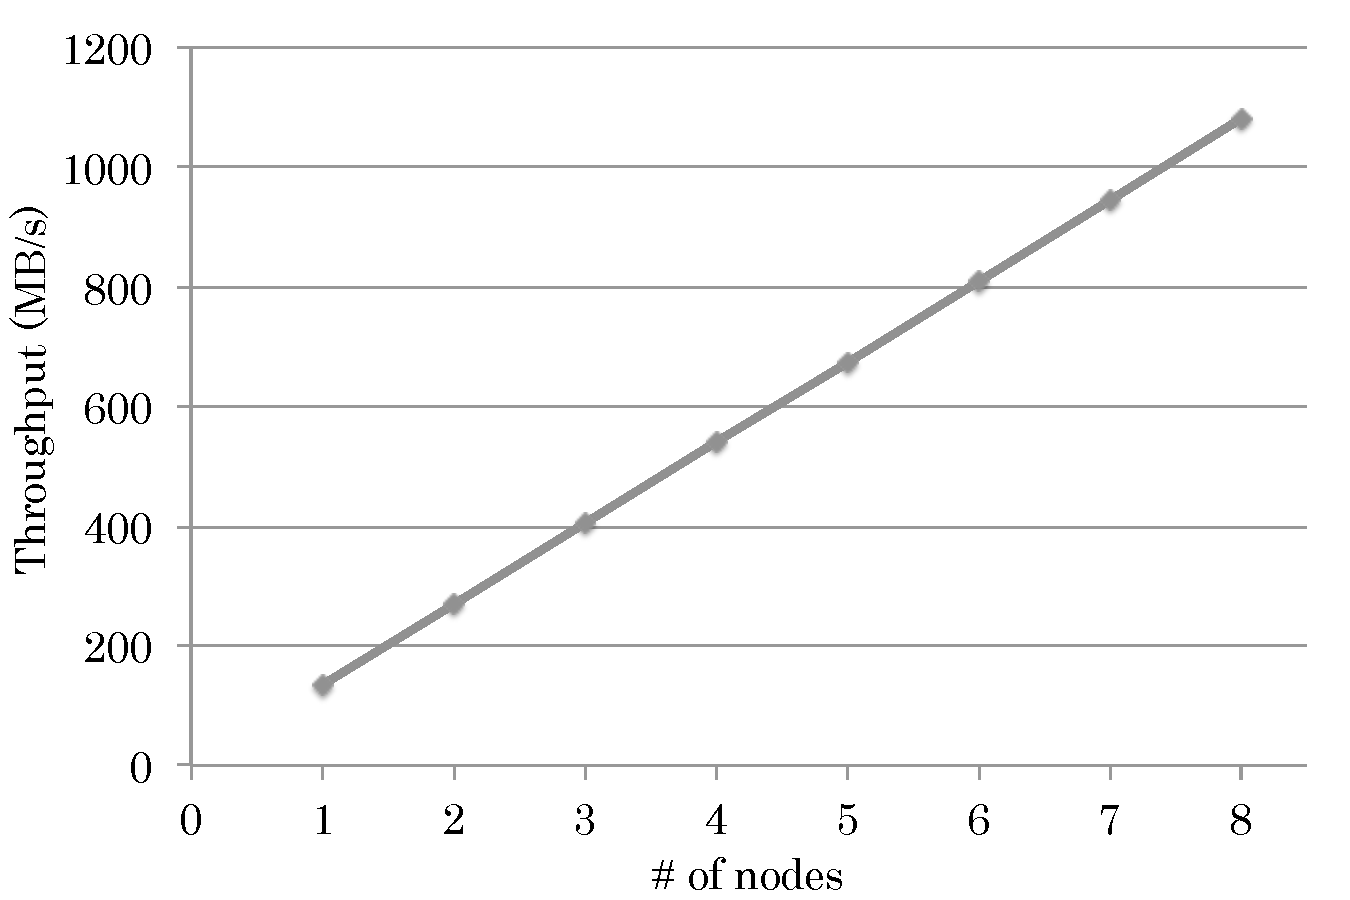
\includegraphics[width=8cm]{img/point_to_point-2}
\caption{Point-to-point communication throughput in Amazon EC2}
\label{background:Amazon point to point throughput}
\end{figure}


% \subsection{Burst Buffer}
% \begin{figure}
% \centering
% 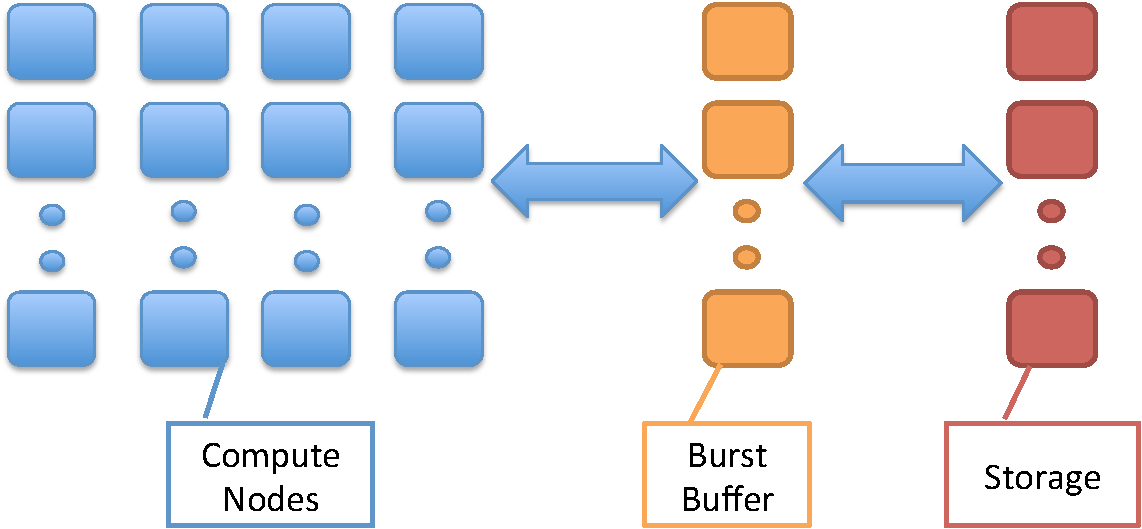
\includegraphics[width=8cm]{img/burst_buffer.pdf}
% \caption{burst buffer architecture}
% \label{background:burst buffer architecture}
% \end{figure}
% 
% Modern high performance systems consist of thousands of compute nodes, and hundreds of
% applications are running at the same time, some I/O request peak can hardly be meet by current
% storage hierarchy. 
% Traditional approach, which solves such problem by providing a higher bandwidth storage will cause
% the storage system under utilization.
% Previous research\cite{on_the_role_of_burst_buffers} proposed a
% burst buffer system as a new tier of current storage hierarchy.
% Burst buffer system uses several local compute nodes as a burst buffer to absorb I/O
% request. 
% By adding such new tier of storage hierarchy, temporal I/O request can be absorb by burst buffer
% without a need of higher bandwidth storage. Figure~.\ref{background:burst buffer architecture}
% shows the architecture of burst buffer.
% 
% Such burst buffer system can burst the application which has a high data locality I/O pattern, since
% the data can be read once from storage and then buffered in the burst buffer system, subsequent
% request for the same data can be accessed from burst buffer.
% Furthermore, applications which write a lot also can benefit from burst buffer system, by buffering
% output data in burst buffer, application can go ahead without waiting data be finally write to
% storage.
% \kento{I think we do not need this subsection or we should combine with the
% previous subsection, because there is no new information from the introduction
% section}


As mentioned in Section \ref{ssec:data_access_locality}, 
a number of data intensive workloads have temporal I/O locality, and their I/O
data can be buffered.
If we can install \emph{large}, \emph{fast} and \emph{shared} buffer space, we
can accelerate these data intensive worklodas.
Motivate by the fact, we innovate the \emph{burst buffer} technology to cloud
environments.
Burst buffer is a new tier in current storage hierarchy for bursty I/O operation
in data intensive applications~\cite{on_the_role_of_burst_buffers} and
checkpointing workloads~\cite{A_User-Level_InfiniBand-Based_File_System_and_Checkpoint_Strategy_for_Burst_Buffers}.
By innovating the new tier of storage, the bursty I/O workloads
can be absorbed without a need of higher bandwidth storage.

Figure \ref{background:Amazon point to point throughput} shows Point-to-point
communication throughput in Amazon EC2. In this evaluation,
we measure the network throughput between a pair of $m3.xlarge$ instances using
Iperf~\cite{iperf}, and increase the number of the pairs. The specification of
the instances is in Table \ref{evaluation:amazon_environment}.
As in the figure, we can see that the network throughput between two nodes is
high and scalable to the increasing number of the pairs.
We take advantage of the high and scalable network throughput to burst I/O
throughput. If we use the memory space of bunch of instances as burst
buffers, we can construct on-demand burst buffer with high throughput
and high scalability on the fly.


% However, when we look at the point to point communication throughput between two compute nodes
% inside Amazon EC2,
% We measure this interconnection network by using Iperf [14].
% \kento{What does the ``inside'' mean ? please describe what did you measure}
% Figure.~\ref{background:amazon throughput} shows a comparison of Amazon Interconnection Network
% throughput and Amazon S3 throughput, although we only show the result up to 8 pairs of nodes
% \kento{Because you did not describe how to measure the performance,
% ``pairs'' is not unknown}, each node achieved only 135MB/s (1GBit/s), the
% influence between nodes is extremely small, figure shows a perfect linear line also a strong scalability.
% \kento{It's too detailed. And Should be mentioned before showing results}.
% When we running the
% benchmark, many other users were also running applications on Amazon, so we can assume that highest
% throughput 1GB/s (8Gbit/s) shown in Figure.~\ref{background:amazon throughput} is not the
% maximum bandwidth of interconnection network in Amazon EC2 \kento{Why do you
% mention this ? If you want to say ``this results is not trustful because other
% applications were running'', please remove this figure and this subsection.
% Instead, you should mention ``Even with other applications are running, the
% performance is still better than S3'' . But, in fat tree topology, almost peak
% throughput can be achieved even if other applications are running like in
% TSUBAME. So I do not think your expectation is true}.
% As Figure.~\ref{background:amazon throughput} shows, Interconnection Network throughput inside
% Amazon EC2 is proportional to numbers of nodes used, on the contrary, Amazon S3 throughput is much
% lower than it, and unstable.
% Also we can find that all nodes access to the same file is slower than access to different file,
% it is because Amazon S3 will distribute different file over machines to
% increase I/O throughput, access to the same file will be limited by S3 server machine bandwidth, and will cause connection
% conflict.
% \kento{Please mention ``so what?''. Why did you compare network(interconnection
% network) and storage(S3) ? People will think this comparison is unfair, and no
% meaning unless you mention that. This subsection looks weird to me because this
% section does not have any ``topic sentence'' and ``so what ?'' sentence}
\subsection{Challenges in Cloud-based Burst Buffers}
\kento{exploiting network for I/O, multiple applications, limited buffer size}
\kento{focus is modeling because \ldots}

